% !TEX root = ../master.tex
\chapter{Implementation}
\label{chap:impl}

The previous chapter yielded a general execution plan that shall implemented in the coming 
section while utilizing the cluster computer at the \ac{DHBW}. 
For each implementation detail the specifically chosen values are given during the process. Each of the steps holds 
the possibilities for errors which will also be evaluated.
The outcome of the taken steps is only a partially functional Hadoop cluster.
The reasons and implications for this restricted outcome are given.
Suggestions for future projects how better results might be achieved is given in the end.

\section{Infrastructure Set-Up in OpenStack}

The foundation for the cluster architecture that has been illustrated in figure \vref{fig:architecture} are the host \acp{VM}, their storage and the network that connects them.
In the course of this process some minor adaptions are made to the proposed architecture.
Especially the \texttt{hadoop-master-0} node now also runs the \ac{HDFS} Datanode and YARN Nodemanager service and therefore has a storage volume attached to it.


To set up the cluster the web interface of OpenStack can be used, which is accessible at
\urlinline{https://controller.c4.dhbw-mannheim.de/} from within the \ac{DHBW} network.
Each operation on the infrastructure can be performed within this interface.

\subsection{Execution}

\subsubsection{Firewall Rules}

TODO sec group considerations, which ports in out? 
default: out is open, in is only ping and ssh on 22
hadoop: detailed view \autocite[][]{hortonworks2017reference}, but for easier development temporary all ports incoming open. most important: 8080 for ambari


\subsubsection{Network}

TODO new internal network chosen from private address space (defined in RFC~1918 by the the Internet Engineering Task Force \autocite[][]{ietf1996rfc1918})

TODO connetio to outside network nedded for general access, (only DH)

TODO describe each of the networks

\begin{table}[hbt]
\resizebox{\textwidth}{!}{%
	\begin{tabular}{lll}
	  Network Name & Sub-networks & Descirption\\
	  \hline
	  ext-net-201 & 141.72.191.0/24 & Pre-configured connection to \ac{DHBW} internal network\\
	  ext-net-112 & 192.168.112.0/20 & Pre-configured connection with unknown destination\\
	  int-net-10 & 10.100.10.0/24 &  New internal network used by Hadoop\\
	\end{tabular}%
	}
	\caption{Sub-networks within the projekt in OpenStack}
	\label{fig:networks_subnets}
\end{table}

\begin{figure}[hbt]
  {\centering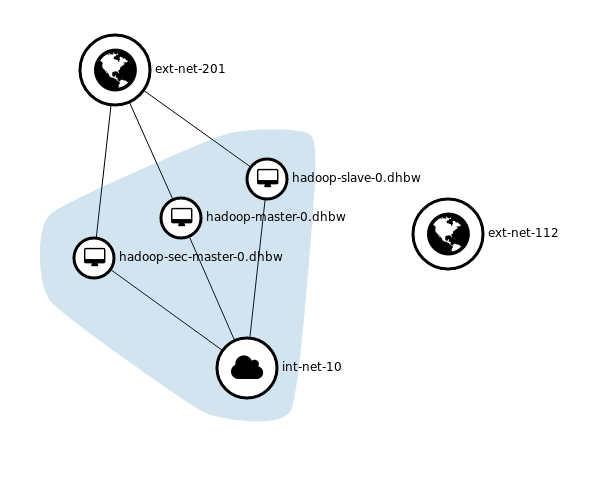
\includegraphics[width=0.8\textwidth]{{img/network_topology}.png}\par}
  \caption{Network topology created in OpenStack}
  \label{fig:network_topology}
\end{figure}


TODO fqdns respective to proposed architecture but with .dhbw ending which is necessary later on

\subsubsection{Virtual Machines}

TODO describe flavors
\ac{VCPU}

\begin{table}[hbt]
\centering
	\begin{tabular}{lrrr}
	  Instance Flavor Name & \acp{VCPU} & \ac{RAM} & Root Disk Size \\
	  \hline
	  m1.nano & 1 & 64~\ac{MB} & 1~\ac{GB} \\
	  m1.tiny & 1 & 512~\ac{MB} & 5~\ac{GB} \\
	  m1.small & 1 & 1~\ac{GB} & 10~\ac{GB} \\
	  m1.medium & 2 & 2~\ac{GB} & 20~\ac{GB} \\
	  m1.large & 4 & 4~\ac{GB} & 40~\ac{GB} \\
	  m1.xlarge & 8 & 8~\ac{GB} & 80~\ac{GB} \\
	\end{tabular}%
	\caption{Available instance sizes in the \ac{DHBW} OpenStack environment}
	\label{fig:instance_sizes}
\end{table}


\begin{table}[hbt]
\centering
	\begin{tabular}{lrl}
	  Resource Type & Amount & Unit\\
	  \hline
	  Instances & 10 & \\
	  \acp{VCPU} & 20 & \\
	  \acs{RAM} & 51200 & \ac{MB} \\
	  Floating \ac{IP} Addresses & 10 & \\
	  Security Groups & 10 & \\
	  Volumes & 10 & \\
	  Volume Storage & 1000 & \ac{GB}
	\end{tabular}%
	\caption{Available resources for the project in the \ac{DHBW} OpenStack environment}
	\label{fig:resources_openstack}
\end{table}


TODO do the math on resources, ratio of cores to ram of 1core:1GB with all flavors above incl small , 
which means with 20 available cores a maximum of 20 GB can be used.
Best solution which maximizes use of resources and created the biggest hosts is as follows
master: xlarge
sec: xlarge
slave:  large

TODO OS: ubuntu 16.04
TODO network attatchment to ext201 and int10+
TODO security group: defualt and hadoop
TODO using ssh key for authentication



\subsubsection{Storage}

TODO
create disks
assing them
format them
ansible will be used to mount them

\subsection{Encountered Issues and Lessons Learned}

TODO Access only from dhbw on site net leads to difficult development conditions where author needs to be on site and is restricted by the locality

TODO Network connection unstable leading to more difficult environment with regular loss of connectivity to server

TODO Internal errors within openstack (temporary) where not enough resources could be allocated to get the requested VMs, later resolved

TODO when encountering resource issues, tried on BW cloud again to train


\section{System Set-Up with Ansible}

TODO ansible script already used in chapter 3 so now it is adapted to the new needs

\subsection{Preparation}

TODO
TODO explain and maybe print this particular playbook yes yes print it with explainations
TODO maybe appendix
TODO Ansible
see \urlinline{https://github.com/XOSplicer/studienarbeit-hadoop-cluster-ansible}
     (in implementation explain how the ansible part works). 
     


\subsection{Execution}

TODO prepare hosts by running setup script
TODO apply ansible playbook
reboot for safty

\subsection{Encountered Issues and Lessons Learned}

TODO
literary none?

\section{Hadoop Set-Up with Ambari}

TODO

TODO Tools will be Apache Spark, Storm, Hive und Pig

\subsection{Preparation}
TODO

\subsection{Execution}
TODO

TODO ,  when promted to select nodes use manual registaration: reason dont upload ssh private key for root access 

\subsection{Encountered Issues and Lessons Learned}
TODO

TODO as expected the larger root partition of 80 GB was enough for the selected services

TODO memory on master node was exceeded even with not all services runnig (only)

TODO network DNS issues lead to failing installation, ha been re-done

TODO services crash due to memory shortage, generel unstable


\section{System Tests}

TODO

\subsubsection{Terasort}

TODO and \autocite{omally2008terasort}
TODO \urlinline{https://hadoop.apache.org/docs/r1.0.4/api/org/apache/hadoop/examples/terasort/TeraGen.html}\\urlinline{https://www.systutorials.com/3235/hadoop-terasort-benchmark/} (also mentioned in \autocite[][]{white2015hadoop})

\subsubsection{Ambari Service Checks}

TODO

HDFS WORKS
YARN is broken (sometimes)
mapred is broken (sometimes)

check successfull where service is up, not all services up. TODO which ones

\section{Conclusion}

TODO dhbw cloud is unreliable af

TODO process is way too hard for and too long for students to do in a lecture without depper understanding of sysadmin  

TODO NOT scuccessfull because of ??????????

TODO Abweichen von architecture war dumm, da memory knapp durch zu viele prozesse

TODO maintainability is fucked, just let professsionals do it


%%%%%%%%%%%%%%%%%%%%
TODO HELP ME IM STREGGELING WITH EXISTENCE





\urlinline{https://gist.github.com/ace-subido/0a9b219b2348921f6a87/3141000d2cbb0f78b967b75304908f4289aa8f01}

\urlinline{https://www.ripublication.com/ijaer18/ijaerv13n6_166.pdf}
\urlinline{http://citeseerx.ist.psu.edu/viewdoc/download?doi=10.1.1.178.1187&rep=rep1&type=pdf}



